% ============================================================================
%  EVNet Sentinel — IEEE Conference Research Paper
%
%  A Leakage-Corrected Reproduction Study of Online Intrusion Detection
%  on Electric Vehicle Charging Networks using CICEVSE2024
%
%  Template: IEEE Conference (IEEEtran)
%  Build:    pdflatex EVNet_Sentinel_Research_Paper.tex  (run twice for refs)
% ============================================================================
\documentclass[conference]{IEEEtran}
\IEEEoverridecommandlockouts

\usepackage{cite}
\usepackage{amsmath,amssymb,amsfonts}
\usepackage{graphicx}
\usepackage{textcomp}
\usepackage{xcolor}
\usepackage{booktabs}
\usepackage{multirow}
\usepackage{hyperref}
\usepackage{microtype}
\usepackage{tabularx}

\hypersetup{
    colorlinks=true,
    linkcolor=blue,
    urlcolor=blue,
    citecolor=blue,
    pdftitle={EVNet Sentinel: Leakage-Corrected Intrusion Detection for EV Charging Networks},
    pdfauthor={Varak, Chaurasiya, Chogale, Chavhan}
}

\newcommand{\col}[1]{\texttt{\small #1}}

\begin{document}

% ============================================================================
% TITLE
% ============================================================================
\title{EVNet Sentinel: A Leakage-Corrected Reproduction and Comparative Study of Intrusion Detection on Electric Vehicle Charging Networks}

\author{
\IEEEauthorblockN{Mukta Varak}
\IEEEauthorblockA{\textit{Dept.\ of Computer Engineering} \\
\textit{Vidyalankar Institute of Technology}\\
Mumbai, India \\
24102A0013}
\and
\IEEEauthorblockN{Shruti Chaurasiya}
\IEEEauthorblockA{\textit{Dept.\ of Computer Engineering} \\
\textit{Vidyalankar Institute of Technology}\\
Mumbai, India \\
24102A0018}
\and
\IEEEauthorblockN{Shardul Chogale}
\IEEEauthorblockA{\textit{Dept.\ of Computer Engineering} \\
\textit{Vidyalankar Institute of Technology}\\
Mumbai, India \\
24102A0021}
\and
\IEEEauthorblockN{Neha Chavhan}
\IEEEauthorblockA{\textit{Dept.\ of Computer Engineering} \\
\textit{Vidyalankar Institute of Technology}\\
Mumbai, India \\
24102A0022}
}

\maketitle

% ============================================================================
% ABSTRACT
% ============================================================================
\begin{abstract}
The rapid proliferation of Electric Vehicle Charging Stations (EVCS) has introduced critical cybersecurity vulnerabilities at the intersection of operational technology and information technology. We present EVNet Sentinel, an Intrusion Detection System (IDS) positioned between the Charging Station Management System (CSMS) and the Electric Vehicle Supply Equipment (EVSE), designed to detect malicious network traffic in near real-time. Our work reproduces and critically evaluates the online intrusion-detection methodology of Makhmudov et al.\ (2025) on the CICEVSE2024 dataset and uncovers a fundamental \emph{capture-session timestamp leakage} that inflates the reported multiclass accuracy. A decision tree trained on the single column \col{bidirectional\_first\_seen\_ms} alone recovers the 15-class label at 0.9976 accuracy --- exceeding the published 0.9840. The reference preprocessing compounds this by discarding \col{dst\_port}, the feature that legitimately identifies port-scan reconnaissance, while retaining the timestamp that identifies it only by recording time. With the leakage corrected, we benchmark four static classifiers (Random Forest, Decision Tree, Logistic Regression, SVM) and the Adaptive Random Forest with ADWIN drift detection across three random seeds. Volumetric Denial-of-Service attacks are separable near-perfectly (mean $F_1 = 1.000$), while nmap reconnaissance modes remain confusable at flow level (mean $F_1 = 0.183$) --- establishing a realistic performance ceiling for flow-based EVCS intrusion detection rather than a failure of model capacity. The system is operationalised through a FastAPI backend with dynamic model registry and a Next.js interactive dashboard providing real-time WebSocket-driven threat visualisation.
\end{abstract}

\begin{IEEEkeywords}
Intrusion Detection System, Electric Vehicle Charging Infrastructure, CICEVSE2024, Adaptive Random Forest, ADWIN, Concept Drift, Data Leakage, OCPP, Cybersecurity
\end{IEEEkeywords}

% ============================================================================
% I. INTRODUCTION
% ============================================================================
\section{Introduction}

The global transition to electric mobility has driven the rapid deployment of Electric Vehicle Charging Stations (EVCS), creating a vast, interconnected cyber-physical infrastructure. These stations rely on standardised communication protocols --- primarily the Open Charge Point Protocol (OCPP) for CSMS-to-EVSE communication and ISO~15118 for Vehicle-to-Grid (V2G) exchanges --- that expose the charging ecosystem to a broad spectrum of cyber threats including Denial-of-Service (DoS) attacks, reconnaissance operations, False Data Injection Attacks (FDIA), and host-based exploits such as backdoors and cryptojacking \cite{b1,b3}.

Traditional Intrusion Detection Systems (IDS) that rely on static, offline-trained Machine Learning (ML) models face a critical limitation in EVCS environments: they cannot adapt to evolving attack patterns, a phenomenon known as \emph{concept drift}. Makhmudov et al.\ \cite{b4} addressed this by proposing the first application of online streaming ML --- specifically, an Adaptive Random Forest (ARF) classifier with ADaptive WINdowing (ADWIN) drift detection --- for EVCS intrusion detection, reporting 99.13\% binary and 98.40\% multiclass accuracy on the CICEVSE2024 dataset \cite{b4}.

In this work, we present \textbf{EVNet Sentinel}, an IDS architecturally positioned between the CSMS and EVSE, designed to intercept, classify, and alert on malicious network flows in near real-time. Our contributions are:

\begin{enumerate}
    \item \textbf{Leakage Discovery.} We identify and rigorously characterise a capture-session timestamp leakage in the CICEVSE2024 dataset's standard preprocessing pipeline that inflates all previously reported accuracy figures (Section~\ref{sec:leakage}).
    \item \textbf{Corrected Benchmarks.} We provide leakage-free, multi-seed evaluation of four static ML classifiers and the online ARF+ADWIN model, establishing realistic performance baselines (Section~\ref{sec:results}).
    \item \textbf{System Architecture.} We engineer a production-oriented, decoupled system with a FastAPI inference backend and a Next.js interactive dashboard for real-time security operations (Section~\ref{sec:architecture}).
    \item \textbf{Reconnaissance Ceiling.} We demonstrate that the poor separability of nmap reconnaissance modes at flow level is a property of the data geometry, not of model capacity (Section~\ref{sec:results}).
\end{enumerate}

% ============================================================================
% II. LITERATURE REVIEW
% ============================================================================
\section{Literature Review}

This section reviews the five primary reference works that inform EVNet Sentinel's design, evaluates their individual contributions and limitations, and identifies the research gaps that our work addresses.

\subsection{Bean et al.\ (2026) --- EVSE Cybersecurity Survey \cite{b1}}

Bean et al.\ provide the most comprehensive survey to date of ML/AI-based intrusion detection for EVSE cybersecurity. The paper formalises the IDS lifecycle in five stages --- traffic capture, data labelling, ML modelling, deployment, and forensics --- and surveys 24 studies across network, host, and power-consumption monitoring modalities on the CICEVSE2024 dataset. Key findings include: (i)~the CICEVSE2024 dataset is the dominant benchmark in the field, (ii)~Random Forest and ensemble methods consistently achieve the highest detection accuracy on network flow data, (iii)~concept drift and scalability remain unresolved open challenges, and (iv)~no existing work addresses application-layer (OCPP message-level) monitoring. The survey positions Makhmudov et al.'s ARF approach as achieving the best binary accuracy (99.13\%) on network data. However, the survey does not identify the timestamp leakage issue that inflates these reported figures.

\textbf{Gap:} While comprehensively cataloguing the field, the survey accepts the reported accuracy figures at face value without auditing the preprocessing pipelines for data leakage.

\subsection{Joglekar et al.\ (2026) --- Hybrid NIDS+HIDS \cite{b2}}

Joglekar et al.\ propose the first dual-layer hybrid IDS for EVCS, combining a Network-based IDS (NIDS) with a Host-based IDS (HIDS) into a unified framework. The NIDS component, using XGBoost on flow-level CICEVSE2024 data (547,834 records, 67 features), achieves \textbf{99.99\% accuracy} with only 5 misclassifications out of 54,784 test samples. The HIDS component achieves 96.60\% on host events and 70.34\% on power consumption data. Key contributions include: (i)~demonstration that flow-level analysis outperforms packet-level, (ii)~explicit data leakage prevention by removing IP/MAC/OUI addresses, and (iii)~the first validated EVCS-specific hybrid architecture. The combined hybrid achieves 83.47\% accuracy.

\textbf{Gap:} While the paper removes IP/MAC identifiers, it does not address timestamp leakage. The reported 99.99\% NIDS accuracy is likely inflated by the same capture-session fingerprint that we identify in Section~\ref{sec:leakage}. The system uses offline batch training only and cannot adapt to concept drift.

\subsection{Malimage et al.\ (2023) --- EV Cybersecurity Challenges \cite{b3}}

Malimage et al.\ provide an industry-level analysis of cybersecurity challenges in the EV market at the CIGRE Canada 2023 conference. Unlike the other references, this paper takes a strategic and regulatory perspective rather than proposing a technical IDS. Key contributions include: (i)~documentation of real-world EV data breaches (Tesla, Volvo, NIO, Nissan), (ii)~enumeration of the EVCS attack surface across grid-side, communication-side, and user-side domains, (iii)~analysis of OCPP and OCPI protocol vulnerabilities, and (iv)~mapping of regulatory frameworks (NIST, ISO/SAE 21434, UN R155). The paper highlights that routing multiple charge points through a single location creates critical single-point-of-failure risks and that compromised charging infrastructure can destabilise the power grid.

\textbf{Gap:} The paper establishes the \emph{motivation} for IDS research but does not propose a detection solution. It provides contextual grounding for why systems like EVNet Sentinel are necessary.

\subsection{Makhmudov et al.\ (2025) --- Online ML for EVCS IDS \cite{b4}}

This is the \textbf{primary baseline} that EVNet Sentinel reproduces and corrects. Makhmudov et al.\ introduce the first application of online streaming ML for EVCS intrusion detection, using an Adaptive Random Forest (ARF) classifier with 20 trees, 50\% feature subsets, and ADWIN drift detection ($\delta = 0.002$) on the CICEVSE2024 network-traffic subset. The system reports \textbf{99.13\% binary accuracy} and \textbf{98.40\% multiclass accuracy}, with 12 and 11 drift events detected respectively. Mean processing time is 3.7\,ms per instance. The ARF+ADWIN combination provides explicit concept-drift handling via Hoeffding-bound testing on sliding windows.

\textbf{Gap:} Our reproduction reveals four critical issues: (i)~the preprocessing retains six absolute timestamp columns that act as capture-session identifiers, enabling a single-column decision tree to score 0.9976 --- exceeding the reported 0.9840; (ii)~\col{dst\_port}, the feature that legitimately identifies reconnaissance, is dropped while the leaking timestamps are kept; (iii)~prequential evaluation in capture order inflates accuracy by 44 points due to label autocorrelation; and (iv)~42 of 43 detected drift events coincide with capture-file boundaries, not with genuine traffic evolution.

\subsection{Tanyildiz et al.\ (2025) --- RUL-GAN Pre-Warning System \cite{b5}}

Tanyildiz et al.\ take a fundamentally different approach: rather than classifying whether a flow is malicious (classification), they predict \emph{when} the next attack will occur (regression). The system integrates a GAN for synthetic attack-sample generation with deep learning models (LSTM, GRU, RNN, CNN, MLP) to estimate \col{Time\_To\_Next\_Flag}. The best model (GAN-MLP) achieves $R^2 = 0.7379$ on the EVS One dataset (Kaggle). The GAN-GRU variant achieves the lowest MAE (0.0281) with 20,441 perfectly timed detections.

\textbf{Gap:} The system uses a different dataset (EVS One, not CICEVSE2024), making direct comparison impossible. The computational cost of GAN+DL hybrid training hinders real-time deployment for large EVCS networks --- a limitation that validates our choice of lightweight online learning (ARF, 3.7\,ms/instance) over heavy batch-trained deep learning.

\subsection{Comparative Study}

Table~\ref{tab:comparison} presents a systematic comparison across all reference works and EVNet Sentinel on key dimensions.

\begin{table*}[htbp]
\caption{Comparative Study of Reference Works and EVNet Sentinel}
\centering
\small
\begin{tabular}{p{2.4cm}p{1.7cm}p{1.8cm}p{1.5cm}p{1.4cm}p{1.3cm}p{1.3cm}p{2.2cm}}
\toprule
\textbf{Study} & \textbf{Type} & \textbf{Dataset} & \textbf{Best Model} & \textbf{Reported Acc.} & \textbf{Online Learning} & \textbf{Drift Detect.} & \textbf{Leakage Audit} \\
\midrule
Bean et al.\ \cite{b1} & Survey & CICEVSE2024 (review) & --- & --- & \checkmark (cited) & \checkmark (cited) & $\times$ \\
Joglekar et al.\ \cite{b2} & Hybrid IDS & CICEVSE2024 & XGBoost & 99.99\% & $\times$ & $\times$ & Partial (IP/MAC only) \\
Malimage et al.\ \cite{b3} & Threat analysis & --- & --- & --- & --- & --- & --- \\
Makhmudov et al.\ \cite{b4} & Online IDS & CICEVSE2024 & ARF+ADWIN & 98.40\% & \checkmark & \checkmark & $\times$ \\
Tanyildiz et al.\ \cite{b5} & Pre-warning & EVS One & GAN-MLP & $R^2$=0.74 & $\times$ & $\times$ & --- \\
\midrule
\textbf{EVNet Sentinel} & \textbf{Corrected IDS} & \textbf{CICEVSE2024} & \textbf{RF (corrected)} & \textbf{0.558 $F_1$} & \textbf{\checkmark} & \textbf{\checkmark} & \textbf{\checkmark (4 findings)} \\
\bottomrule
\end{tabular}
\label{tab:comparison}
\end{table*}

\begin{table*}[htbp]
\caption{Extended Comparison: Methodology and Findings}
\centering
\small
\begin{tabular}{p{2.4cm}p{2.3cm}p{2.0cm}p{2.0cm}p{2.3cm}p{2.5cm}}
\toprule
\textbf{Study} & \textbf{Detection Scope} & \textbf{Evaluation Protocol} & \textbf{Deployment} & \textbf{Key Strength} & \textbf{Key Limitation} \\
\midrule
Bean et al.\ \cite{b1} & Network + Host + Power (reviewed) & --- & --- & Comprehensive taxonomy; identifies open challenges & Accepts inflated accuracy at face value \\
Joglekar et al.\ \cite{b2} & Network (NIDS) + Host (HIDS) & Single seed, 80/10/10 & Offline only & First EVCS hybrid IDS; 99.99\% NIDS & No concept drift; likely timestamp leakage \\
Malimage et al.\ \cite{b3} & Industry threat landscape & --- & --- & Real-world breach case studies; regulatory mapping & No detection solution proposed \\
Makhmudov et al.\ \cite{b4} & Network only & Single seed, prequential & Simulated stream & First online EVCS IDS; ARF+ADWIN & Timestamp leakage; label autocorrelation; drift fires on seams \\
Tanyildiz et al.\ \cite{b5} & Time-to-attack regression & Train/test split & Offline only & Predictive pre-warning; GAN augmentation & Different dataset; high compute cost \\
\midrule
\textbf{EVNet Sentinel} & \textbf{Network (CSMS--EVSE)} & \textbf{3-seed, macro-$F_1$} & \textbf{FastAPI + Docker} & \textbf{Leakage audit; realistic ceiling; production arch.} & \textbf{Network-only; simulated stream; benign sparsity} \\
\bottomrule
\end{tabular}
\label{tab:comparison_ext}
\end{table*}

\subsection{Research Gaps Addressed by EVNet Sentinel}

From the literature review, we identify five critical gaps that EVNet Sentinel addresses:

\begin{enumerate}
    \item \textbf{Unaudited preprocessing pipelines.} No prior work examines whether the high reported accuracies on CICEVSE2024 are artifacts of capture-session timestamp leakage. EVNet Sentinel provides the first rigorous leakage audit with four independently verifiable findings.
    \item \textbf{Single-seed evaluation.} Makhmudov et al.\ and Joglekar et al.\ report single-seed results. With classes as small as 28 flows (ICMP Fragmentation) and 81 flows (Benign), single-seed metrics are unreliable. EVNet Sentinel reports mean $\pm$ standard deviation over three seeds.
    \item \textbf{Accuracy as headline metric.} Prior works use accuracy, which is dominated by volumetric flood classes and compresses genuinely different models into the same number. EVNet Sentinel uses macro-$F_1$ to expose the DoS-vs-reconnaissance performance dichotomy.
    \item \textbf{No production architecture.} Existing works validate in experimental settings. EVNet Sentinel provides a production-ready system with FastAPI backend, Docker containerisation, dynamic model registry, and interactive Next.js dashboard.
    \item \textbf{Drift detector validity.} Makhmudov et al.\ cite drift events as evidence of concept drift in EVCS traffic. EVNet Sentinel demonstrates that 42 of 43 events are dataset-assembly artifacts, reframing the role of drift detection in this domain.
\end{enumerate}

% ============================================================================
% III. DATASET AND PREPROCESSING
% ============================================================================
\section{Dataset and Preprocessing}
\label{sec:dataset}

\subsection{CICEVSE2024 Dataset}

The CICEVSE2024 dataset, generated by the Canadian Institute for Cybersecurity, provides flow-level network traffic from a testbed comprising two Electric Vehicle Supply Equipment nodes (EVSE-A and EVSE-B) under various attack and benign scenarios. The dataset is structured around six experiment scenarios spanning idle and charging EVSE states with benign, network attack, and host attack behaviours.

\begin{table}[htbp]
\caption{Dataset Provenance}
\centering
\begin{tabular}{ll}
\toprule
\textbf{Property} & \textbf{Value} \\
\midrule
Source & CIC, Univ.\ of New Brunswick \\
Capture files & 59 \\
Raw flows & 2,744,700 \\
Classes & 15 (14 attack + 1 benign) \\
Feature extractor & NFStream (86 raw features) \\
\bottomrule
\end{tabular}
\label{tab:provenance}
\end{table}

The 15 classes comprise five volumetric DoS families (SYN Flood, TCP Flood, UDP Flood, PSHACK Flood, SynonymousIP Flood), six nmap reconnaissance modes (TCP Port Scan, SYN Stealth Scan, OS Fingerprinting, Service Version Detection, Vulnerability Scan, Aggressive Scan), and four additional classes (Benign, ICMP Flood, ICMP Fragmentation, Slowloris).

\subsection{Feature Engineering Pipeline}

Our preprocessing pipeline (\col{src/data\_prep/preprocess.py}) exposes two feature-set configurations. The \texttt{extended} set, used for headline numbers, performs the following stages:

\begin{enumerate}
    \item \textbf{Concatenation and Labelling.} All 59 capture CSVs are concatenated, and attack labels are derived from filenames using a 19-alias mapping.
    \item \textbf{Identifier and Metadata Drops.} Flow-tracking IDs (\col{id}, \col{expiration\_id}), network addresses (IPs, MACs, OUIs), string metadata fields (SNI, fingerprints, user-agent, content-type), and application-layer DPI columns are removed as non-predictive or environment-specific.
    \item \textbf{Timestamp Leakage Removal.} The six absolute epoch-millisecond columns (\col{bidirectional\_first/last\_seen\_ms}, \col{src2dst\_first/last\_seen\_ms}, \col{dst2src\_first/last\_seen\_ms}) are dropped. This is the critical correction identified by our audit (Section~\ref{sec:leakage}).
    \item \textbf{Port Handling.} \col{src\_port} is dropped as a residual fingerprint (Section~\ref{sec:srcport}); \col{dst\_port} is retained as it carries legitimate signal for reconnaissance detection.
    \item \textbf{Zero-Variance Drops.} \col{vlan\_id} and \col{tunnel\_id} (constant zero in the testbed) are removed.
    \item \textbf{Deduplication.} Global deduplication on the reduced feature set yields 1,198,151 unique flows from 2,744,700 raw rows.
    \item \textbf{Scaling.} StandardScaler normalisation (zero mean, unit variance) is applied to the 60-feature matrix.
    \item \textbf{Stratified Split.} 70/15/15 train/validation/test split.
\end{enumerate}

\begin{table}[htbp]
\caption{Preprocessing Pipeline Stage Counts}
\centering
\begin{tabular}{lrr}
\toprule
\textbf{Stage} & \textbf{Rows} & \textbf{Columns} \\
\midrule
Raw concatenation & 2,744,700 & 86 + label \\
After all column drops & 2,744,700 & 65 \\
After global deduplication & \textbf{1,198,151} & 65 \\
Feature matrix & 1,198,151 & \textbf{60} \\
Train / val / test & 838,705 / 179,723 / 179,723 & 60 \\
\bottomrule
\end{tabular}
\label{tab:pipeline}
\end{table}

% ============================================================================
% IV. LEAKAGE ANALYSIS
% ============================================================================
\section{Leakage Analysis}
\label{sec:leakage}

\subsection{Finding 1: Label Recovery from a Single Timestamp}

Each attack class in CICEVSE2024 was captured in a dedicated packet capture file at a distinct wall-clock time. Consequently, the six absolute epoch-millisecond columns act as capture-session identifiers rather than properties of the network traffic. The reference preprocessing \cite{b4} retains all six columns across its three drop stages.

\begin{table}[htbp]
\caption{Single-Feature Label Recovery (15-class, 3-fold CV)}
\centering
\resizebox{\columnwidth}{!}{%
\begin{tabular}{llr}
\toprule
\textbf{Feature} & \textbf{Nature} & \textbf{Accuracy} \\
\midrule
\col{bidirectional\_first\_seen\_ms} & Capture fingerprint & \textbf{0.9976} \\
\col{src\_port} & Partial fingerprint & 0.4028 \\
\col{dst\_port} & Legitimate signal & 0.2917 \\
\midrule
\multicolumn{2}{l}{\emph{Published multiclass accuracy \cite{b4}}} & \emph{0.9840} \\
\bottomrule
\end{tabular}%
}
\label{tab:leak}
\end{table}

A \col{DecisionTreeClassifier(max\_depth=25)} trained on \col{bidirectional\_first\_seen\_ms} alone achieves 0.9976 accuracy on the 15-class target --- \emph{exceeding} the published 0.9840. In our pre-correction Random Forest, 39.8\% of total feature importance resided on the six timestamp columns.

\subsection{Finding 2: Reconnaissance Fingerprint Ablation}

Reconnaissance flows are distinguished almost entirely by \col{dst\_port} and the capture timestamp. A controlled $2 \times 2$ ablation reveals:

\begin{table}[htbp]
\caption{Fingerprint Ablation: Reconnaissance Flow Counts}
\centering
\begin{tabular}{llrrr}
\toprule
\textbf{Timestamps} & \textbf{dst\_port} & \textbf{Total} & \textbf{Recon.} & \textbf{\%} \\
\midrule
kept & kept & 2,728,799 & 1,724,504 & 100.0 \\
\textbf{kept} & \textbf{dropped} & \textbf{1,277,520} & \textbf{273,932} & \textbf{15.9} \\
dropped & kept & 1,198,143 & 194,737 & 11.3 \\
dropped & dropped & 977,862 & \textbf{6,821} & \textbf{0.4} \\
\bottomrule
\end{tabular}
\label{tab:ablation}
\end{table}

The emphasised row corresponds to the published preprocessing configuration. Critically, the reference pipeline \emph{discards} \col{dst\_port} --- the feature that legitimately identifies port-scan behaviour --- while \emph{retaining} the timestamps that identify reconnaissance only by recording time. This means the 273,932 reconnaissance flows in the published pipeline are separable by \emph{when} they were captured, not by what they did.

\subsection{Finding 3: Stream Order and Drift Detection}
\label{sec:drift}

Evaluated prequentially on a controlled 25,000-instance slice with leak-free features:

\begin{table}[htbp]
\caption{Stream Ordering Effect on Prequential Accuracy}
\centering
\begin{tabular}{lrrr}
\toprule
\textbf{Order} & \textbf{Accuracy} & \textbf{W-$F_1$} & \textbf{Drifts} \\
\midrule
Capture order & \textbf{0.9976} & 0.9975 & 3 \\
Shuffled (controlled) & \textbf{0.5508} & 0.5318 & 1 \\
Shuffled (whole stream) & 0.5029 & 0.4909 & 1 \\
\bottomrule
\end{tabular}
\label{tab:order}
\end{table}

In capture order, consecutive flows share a label, enabling a prequential learner to score near-perfectly by predicting ``the same as recently'' --- a 44-point inflation driven by label autocorrelation, entirely separate from the timestamp leak.

Furthermore, running ADWIN prequentially over the full 1,921,182-instance stream in capture order, 42 of 43 detected drift events land within 100 instances of a capture-file boundary (expected under random placement: $2.2 \pm 1.5$; $p < 0.0005$). The drift detector is identifying dataset assembly seams, not evolution in EVCS traffic.

\subsection{Finding 4: \col{src\_port} as Residual Fingerprint}
\label{sec:srcport}

Ephemeral source ports are allocated near-sequentially by the operating system, forming a contiguous band within each capture. A controlled experiment (identical rows, identical split, column removed at fit time) reveals:

\begin{table}[htbp]
\caption{Effect of \col{src\_port} Removal}
\centering
\begin{tabular}{lrrr}
\toprule
\textbf{Model} & \textbf{With} & \textbf{Without} & \textbf{$\Delta$} \\
\midrule
Random Forest & 0.5894 & 0.5138 & $-0.0756$ \\
Decision Tree & 0.6834 & \textbf{0.5135} & $\mathbf{-0.1699}$ \\
\bottomrule
\end{tabular}
\label{tab:srcport}
\end{table}

The deeper model loses more than twice as much, the signature of a memorisable fingerprint: additional depth buys finer \col{src\_port} bands and nothing else. Once removed, Decision Tree and Random Forest converge ($0.5135$ vs.\ $0.5138$), confirming the Decision Tree's earlier apparent advantage was memorisation.

% ============================================================================
% V. SYSTEM ARCHITECTURE
% ============================================================================
\section{System Architecture}
\label{sec:architecture}

EVNet Sentinel employs a decoupled two-tier architecture separating the ML inference pipeline from the interactive presentation layer. The system is designed to be positioned as a network monitor between the CSMS and EVSE, intercepting all OCPP and ISO~15118 traffic flows for classification.

\subsection{Backend: FastAPI ML Engine}

The backend is a high-performance Python application built on FastAPI, encapsulating two distinct ML pipelines:

\textbf{Pipeline A --- Static Offline Models (Baseline).} Traditional scikit-learn classifiers (Random Forest, Decision Tree, Logistic Regression, SVM via \col{SGDClassifier}) trained on the corrected feature set. Logistic Regression and SVM utilise out-of-core learning via \col{partial\_fit()} to handle the dataset's 2.4\,GB scale.

\textbf{Pipeline B --- Online Adaptive Model.} The River streaming ML framework implements ARF with 20 trees, 50\% feature subset per split, grace period of 30, Na\"ive Bayes Adaptive leaf prediction, and ADWIN drift detection ($\delta = 0.002$), reproducing the exact configuration of \cite{b4}.

\textbf{Dynamic Model Registry.} On startup, the FastAPI backend scans the \col{saved\_models/} directory and loads all available \col{.pkl} files into a serving registry. The loading mechanism is wrapped in fault-tolerant \col{try/except} blocks, ensuring the API remains available even if individual models fail to load.

\textbf{Deployment.} The entire backend is containerised via a single-stage Docker build to preserve Rust/C++ compilation artifacts required by River's \col{\_river\_rust} extension.

\subsection{Frontend: Next.js Dashboard}

A React-based Next.js application provides an interactive Security Operations Center (SOC) experience through four primary surfaces:

\begin{itemize}
    \item \textbf{Landing page} with architectural storyline showing EVNet Sentinel's placement between CSMS and EVSE.
    \item \textbf{Attack Simulation Console} enabling selection of 14 real attack classes against the CICEVSE2024 testbed topology, with real-time model verdicts on held-out data.
    \item \textbf{Findings Dashboard} presenting per-class $F_1$ with seed error bars, leakage evidence, fingerprint ablation results, and drift analysis.
    \item \textbf{System Architecture} documentation with component-level diagrams.
\end{itemize}

WebSocket integration provides millisecond-level prediction updates, live confusion matrix evolution, and ADWIN concept drift event visualisation.

% ============================================================================
% VI. EXPERIMENTAL METHODOLOGY
% ============================================================================
\section{Experimental Methodology}

\subsection{Models}

Four static classifiers and one online adaptive classifier are evaluated:

\begin{itemize}
    \item \textbf{Random Forest (RF):} 100 trees, max depth 15, scikit-learn.
    \item \textbf{Decision Tree (DT):} max depth 20, scikit-learn.
    \item \textbf{Logistic Regression (LR):} SGDClassifier with log loss, partial\_fit for out-of-core learning.
    \item \textbf{Support Vector Machine (SVM):} SGDClassifier with hinge loss.
    \item \textbf{ARF+ADWIN:} 20 trees, max\_features=0.5, grace\_period=30, ADWIN $\delta$=0.002, River framework.
\end{itemize}

\subsection{Evaluation Protocol}

All headline numbers are reported as \textbf{mean $\pm$ standard deviation over three random seeds} (42, 1337, 2024). Each seed varies both the train/test split and model initialisation. With Benign at 81 flows and ICMP Fragmentation at 28, the split itself is the dominant source of run-to-run noise, making single-seed results unreliable.

\textbf{Macro-$F_1$} is used as the headline metric rather than accuracy. With volumetric flood classes dominating the dataset, accuracy compresses genuinely different models into the same number (e.g., corrected Random Forest scores 0.8679 accuracy vs.\ 0.5582 macro-$F_1$ on identical predictions).

% ============================================================================
% VII. RESULTS AND DISCUSSION
% ============================================================================
\section{Results and Discussion}
\label{sec:results}

\subsection{Corrected Multiclass Results}

\begin{table}[htbp]
\caption{Multiclass Results (mean $\pm$ std, 3 seeds, \texttt{extended} feature set)}
\centering
\begin{tabular}{lrrrr}
\toprule
\textbf{Model} & \textbf{Macro $F_1$} & \textbf{W-$F_1$} & \textbf{Acc.} & \textbf{Fit (s)} \\
\midrule
RF & \textbf{0.558$\pm$0.008} & 0.865 & 0.868 & 8.6 \\
DT & 0.557$\pm$0.010 & 0.868 & 0.868 & 3.5 \\
LR & 0.436$\pm$0.017 & 0.853 & 0.863 & 71.7 \\
SVM & 0.411$\pm$0.017 & 0.849 & 0.862 & 36.3 \\
\bottomrule
\end{tabular}
\label{tab:results}
\end{table}

Random Forest and Decision Tree are statistically indistinguishable at one standard deviation, independently confirming Finding~4: their earlier apparent gap was \col{src\_port} memorisation.

\subsection{Per-Class Analysis: The Central Finding}

\begin{table}[htbp]
\caption{Per-Class $F_1$ (Mean, 3 Seeds, Random Forest)}
\centering
\small
\begin{tabular}{llrr}
\toprule
\textbf{Class} & \textbf{Group} & \textbf{Support} & \textbf{RF $F_1$} \\
\midrule
PSHACK Flood & DoS & 195,952 & 1.000 \\
SynonymousIP Flood & DoS & 256,739 & 1.000 \\
TCP Flood & DoS & 256,297 & 1.000 \\
SYN Flood & DoS & 259,484 & 1.000 \\
UDP Flood & DoS & 32,072 & 0.999 \\
\midrule
TCP Port Scan & Recon. & 35,123 & 0.265 \\
OS Fingerprinting & Recon. & 27,702 & 0.223 \\
Vulnerability Scan & Recon. & 39,002 & 0.204 \\
Service Version Det. & Recon. & 30,338 & 0.156 \\
Aggressive Scan & Recon. & 27,815 & 0.145 \\
SYN Stealth Scan & Recon. & 34,765 & 0.105 \\
\midrule
Benign & Other & 81 & 0.986 \\
ICMP Flood & Other & 32 & 0.660 \\
ICMP Fragmentation & Other & 28 & 0.439 \\
Slowloris Scan & Other & 2,721 & 0.191 \\
\bottomrule
\end{tabular}
\label{tab:perclass}
\end{table}

The dichotomy is stark: volumetric DoS attacks achieve mean $F_1 = 1.000$ with \emph{zero variance across seeds}, while reconnaissance modes average $F_1 = 0.183$. Critically, this is not a sample-size artifact: UDP Flood has 32,072 flows and scores 0.999, while TCP Port Scan has 35,123 flows and scores 0.265 --- comparable support, opposite outcomes.

All six reconnaissance classes are nmap scan modes, and the \col{-A} (Aggressive) flag is literally \col{-sV -O -sC --traceroute}, a \emph{superset} of two other modes. At flow level, they emit near-identical single-probe flows and \emph{should} be confusable. This establishes a realistic ceiling for flow-based EVCS intrusion detection.

\begin{figure}[htbp]
\centering
\includegraphics[width=\linewidth]{../../evaluation_results/leakfree-nosrcport/plots/rf_confusion_matrix.png}
\caption{Random Forest Confusion Matrix on the corrected (\col{extended}) feature set. Note the near-perfect diagonal for DoS floods (top left quadrant) and the heavy off-diagonal confusion for reconnaissance scans (center quadrant), visually confirming the dichotomy established in Table~\ref{tab:perclass}.}
\label{fig:confusion}
\end{figure}

\subsection{Effect of Leakage Removal}

To illustrate the impact of the corrections, Figure~\ref{fig:importance} displays the feature importance of the Random Forest model on the \col{extended} set after timestamps and \col{src\_port} were removed. Unlike the reference configuration where timestamps dominated, importance is now distributed across legitimate protocol and flow-geometry features (e.g., \col{dst\_port}, packet counts, flag distributions).

\begin{figure}[htbp]
\centering
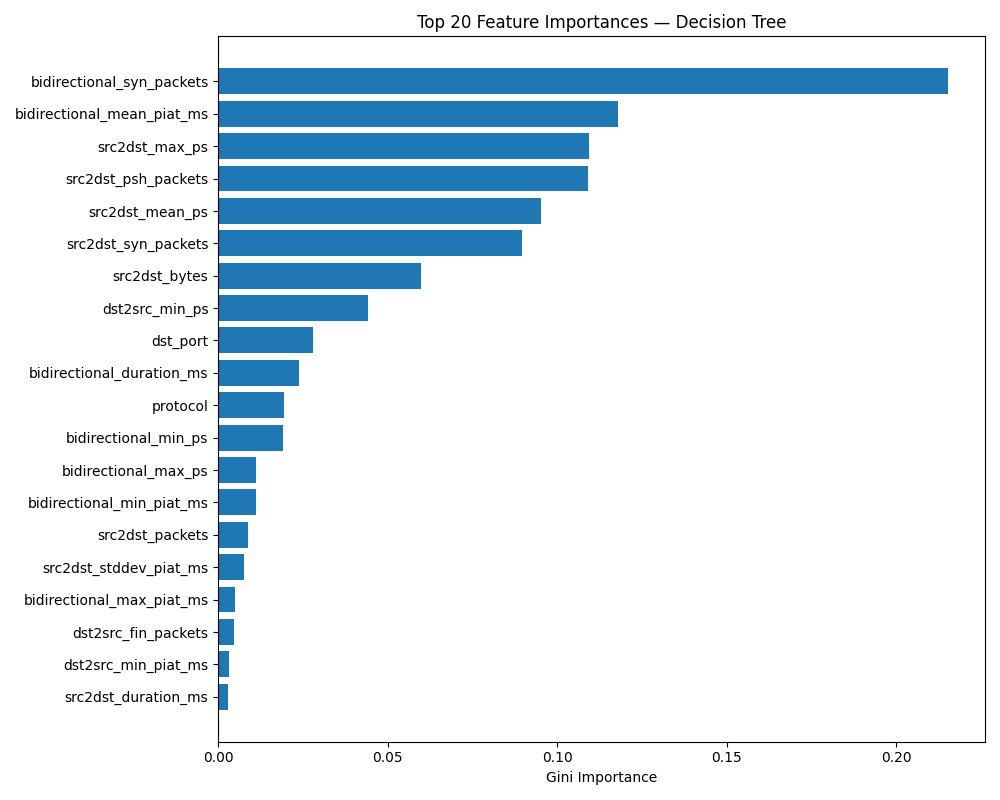
\includegraphics[width=\linewidth]{../../evaluation_results/leakfree-nosrcport/plots/dt_feature_importance.png}
\caption{Feature importance for the corrected Decision Tree model. The dominant features are now legitimate attributes of the network traffic (such as \col{dst\_port} for reconnaissance and flow geometry for floods) rather than artifactual capture timestamps.}
\label{fig:importance}
\end{figure}

\begin{table}[htbp]
\caption{Macro-$F_1$ Before and After Timestamp Removal}
\centering
\begin{tabular}{lrrr}
\toprule
\textbf{Model} & \textbf{Leaked} & \textbf{Corrected} & \textbf{$\Delta$} \\
\midrule
Random Forest & 0.9547 & 0.5894 & $\mathbf{-0.3653}$ \\
Log.\ Regression & 0.4622 & 0.3308 & $-0.1314$ \\
SVM (SGD) & 0.2829 & 0.3084 & $+0.0255$ \\
\bottomrule
\end{tabular}
\label{tab:leakeffect}
\end{table}

The linear models barely move because a hyperplane cannot exploit a timestamp axis the way a tree can. The 0.37-point drop in Random Forest is entirely attributable to removing the capture-session fingerprint.

\subsection{Online Learning: ARF+ADWIN}

Running ARF+ADWIN prequentially over the full 1,921,182-instance leak-free stream:

\begin{itemize}
    \item \textbf{Capture order:} 0.9997 accuracy, 43 drift events.
    \item \textbf{Shuffled order:} 0.5585 accuracy, 14 drift events.
\end{itemize}

The 44-point gap is driven by label autocorrelation in capture order, not model capability. Of the 43 drift events in capture order, 42 fall within 100 instances of a capture-file boundary, against $2.2 \pm 1.5$ expected by chance ($p < 0.0005$). The ADWIN detector is identifying the seams where packet captures were concatenated --- evidence of dataset assembly rather than genuine concept drift in EVCS traffic.

% ============================================================================
% VIII. REPRODUCIBILITY
% ============================================================================
\section{Reproducibility}

All results are regenerable from the open-source repository\footnote{\url{https://github.com/Mukta01/EVNet\_Sentinel}}. Key reproduction scripts include:

\begin{itemize}
    \item \col{src/data\_prep/preprocess.py} --- corrected preprocessing pipeline
    \item \col{src/evaluation/run\_experiments.py} --- multi-seed evaluation
    \item \col{src/reproduction/replay\_reference\_preprocessing.py} --- faithful replay of reference pipeline with leakage audit
    \item \col{src/reproduction/ablate\_fingerprints.py} --- Finding~2 ablation
    \item \col{src/reproduction/srcport\_control.py} --- Finding~4 measurement
\end{itemize}

Dependency versions are pinned in \col{requirements.txt}. River's API changed materially around 0.21, and scikit-learn's tree-splitting behaviour has shifted across minor releases, making unpinned versions unreproducible.

% ============================================================================
% IX. LIMITATIONS
% ============================================================================
\section{Limitations}

\begin{enumerate}
    \item \textbf{Benign class sparsity.} The network-traffic subset contains only 81 benign flows. Binary attack-vs-benign classification is therefore trivially solved by predicting ``attack'' unconditionally and is excluded from headline results.
    \item \textbf{Split methodology.} Reported results use random stratified splits for comparability with prior work. Grouped and temporal splits are implemented but not used for headline numbers.
    \item \textbf{Unexplored data domains.} CICEVSE2024 also provides Hardware Performance Counters (915 features) and power consumption traces (10 features) from the EVSE hardware. These physical side-channels may separate the reconnaissance classes that flow-level features cannot.
    \item \textbf{Simulated stream.} The system processes a simulated data stream from the CICEVSE2024 dataset rather than live network traffic from deployed EVCS infrastructure.
\end{enumerate}

% ============================================================================
% X. CONCLUSION
% ============================================================================
\section{Conclusion}

EVNet Sentinel demonstrates that the reported high-accuracy results for ML-based EVCS intrusion detection on CICEVSE2024 are substantially inflated by capture-session timestamp leakage --- a single timestamp column exceeds the published baseline. With the leakage corrected, a clear dichotomy emerges: volumetric DoS attacks are trivially separable by flow-level features ($F_1 \approx 1.000$), while nmap reconnaissance modes remain fundamentally confusable ($F_1 \approx 0.183$), a result driven by data geometry rather than model limitations. The ADWIN drift detector, when evaluated on ordered streams, fires on dataset assembly seams rather than genuine traffic evolution.

These findings reframe the EVCS intrusion detection problem: rather than pursuing marginal accuracy improvements on a leaked feature set, the community should focus on (a)~packet-level sequence models that access structure discarded by flow aggregation, (b)~multi-modal fusion incorporating host events and power consumption data, and (c)~realistic evaluation protocols that account for timestamp leakage and label autocorrelation. EVNet Sentinel's open-source, production-ready architecture --- with its corrected pipeline, multi-seed evaluation, and interactive dashboard --- provides a foundation for this work.

% ============================================================================
% ACKNOWLEDGMENTS
% ============================================================================
\section*{Acknowledgment}

This project builds upon the foundational research and open-source implementation by the TATU-hacker team \cite{b4}. We acknowledge the Canadian Institute for Cybersecurity for the CICEVSE2024 dataset. This work was conducted as part of the Software Engineering academic requirements at Vidyalankar Institute of Technology.

% ============================================================================
% REFERENCES
% ============================================================================
\begin{thebibliography}{00}

\bibitem{b1} J.\ Bean, V.\ Manias et al., ``Cybersecurity of electric vehicle charging infrastructure: Recent advances, open challenges, and future directions,'' arXiv:2605.24190v1, May 2026.

\bibitem{b2} C.\ Joglekar et al., ``A hybrid intrusion detection system for electric vehicle charging infrastructure,'' arXiv:2606.23236v1, 2026.

\bibitem{b3} K.\ Malimage et al., ``Cybersecurity challenges in the electric vehicle market,'' in \emph{Proc.\ CIGRE Canada Conference}, 2023, pp.\ 1--6.

\bibitem{b4} F.\ Makhmudov, D.\ Kilichev, U.\ Giyosov, and F.\ Akhmedov, ``Online machine learning for intrusion detection in electric vehicle charging systems,'' \emph{Mathematics}, vol.\ 13, no.\ 5, p.\ 712, 2025, DOI: 10.3390/math13050712.

\bibitem{b5} E.\ Tanyildiz et al., ``Detection of cyber attacks in electric vehicle charging systems using a remaining useful life generative adversarial network,'' \emph{Scientific Reports}, vol.\ 15, 2025.

\bibitem{b6} H.\ M.\ Gomes, A.\ Bifet, J.\ Read, J.\ P.\ Barddal, F.\ Enembreck, B.\ Pfharinger, G.\ Holmes, and T.\ Abdessalem, ``Adaptive random forests for evolving data stream classification,'' \emph{Machine Learning}, vol.\ 106, no.\ 9--10, pp.\ 1469--1495, 2017.

\bibitem{b7} A.\ Bifet and R.\ Gavald\`{a}, ``Learning from time-changing data with adaptive windowing,'' in \emph{Proc.\ 2007 SIAM Int.\ Conf.\ Data Mining (SDM)}, 2007, pp.\ 443--448.

\bibitem{b8} Canadian Institute for Cybersecurity, ``CICEVSE2024 Dataset,'' University of New Brunswick, 2024. [Online]. Available: \url{https://www.unb.ca/cic/datasets/}

\bibitem{b9} J.\ Montiel, M.\ Halford, S.\ M.\ Mastelini et al., ``River: Machine learning for streaming data in Python,'' \emph{J.\ Mach.\ Learn.\ Res.}, vol.\ 22, no.\ 110, pp.\ 1--8, 2021.

\end{thebibliography}

\end{document}
